\section{Auswertung}
\label{sec:Auswertung}
Allgemeine Rechnungen wurden mit der python-Bibliothek numpy [4] automatisiert.
Die graphischen Unterstützungen wurden mit Hilfe der python-Bibliothek matplotlib [2]
erstellt.
\subsection{Bestimmung der Strömungsgeschwindigkeit der Dopplerflüssgkeit} \label{sub:velocity}
Mit Hilfe der Gleichung $REFERENZ$ lässt sich die Strömungsgeschwindigkeit der Dopplerflüssgkeit bestimmen.
Zu den verschiedenen Rohrdurchmessern ($D_\text{groß} = \SI{16}{\milli\metre}$, $D_\text{mittel} = \SI{10}{\milli\metre}$,
$D_\text{klein} = \SI{7}{\milli\metre}$) sind die zu den Umdrehungen gemessenen Frequenzverschiebungen $\symup{\Delta} \nu$,
und die daraus errechneten Strömungsgeschwindigkeiten  in den Tabellen \ref{tab:big}, \ref{tab:middle} und \ref{tab:tiny} aufgetragen.
\begin{table}
    \centering
    \caption{Gemessene Frequenzverschiebungen
            und die daraus errechneten Strömungsgeschwindigkeiten ($D_\text{groß} = \SI{16}{\milli\metre}$)}
    \label{tab:big}
    \begin{tabular}{S[table-format=4.0]
                    S[table-format=2.0] S[table-format=1.3] 
                    S[table-format=3.0] S[table-format=2.3] 
                    S[table-format=3.0] S[table-format=2.3]}
        \toprule
        &
        \multicolumn{2}{c}{$\theta = \ang{15;;}$} &
        \multicolumn{2}{c}{$\theta = \ang{30;;}$} & 
        \multicolumn{2}{c}{$\theta = \ang{60;;}$} \\
        \cmidrule(lr){2-3} \cmidrule(lr){4-5} \cmidrule(lr){6-7}
        {$\text{rpm}$}&
        {$\symup{\Delta} \nu \mathbin{/} \si{\hertz}$} & {$v \mathbin{/} \si{\milli\meter\second\tothe{-1}}$} & 
        {$\symup{\Delta} \nu \mathbin{/} \si{\hertz}$} & {$v \mathbin{/} \si{\milli\meter\second\tothe{-1}}$} &
        {$\symup{\Delta} \nu \mathbin{/} \si{\hertz}$} & {$v \mathbin{/} \si{\milli\meter\second\tothe{-1}}$} \\
        \midrule
        5400 & 49 & 24.366 & 73  & 18.790 & 110 & 16.347\\
        6200 & 61 & 30.333 & 98  & 25.225 & 146 & 21.697\\
        7000 & 73 & 36.300 & 116 & 29.858 & 183 & 27.196\\
        7800 & 85 & 42.267 & 122 & 31.403 & 208 & 30.911\\
        8400 & 98 & 48.731 & 159 & 40.927 & 250 & 37.152\\
    \end{tabular}
\end{table}
\begin{table}
    \centering
    \caption{Gemessene Frequenzverschiebungen
            und die daraus errechneten Strömungsgeschwindigkeiten ($D_\text{mittel} = \SI{10}{\milli\metre}$)}
    \label{tab:middle}
    \begin{tabular}{S[table-format=4.0]
                    S[table-format=3.0] S[table-format=2.3] 
                    S[table-format=3.0] S[table-format=2.3] 
                    S[table-format=3.0] S[table-format=3.3]}
        \toprule
        &
        \multicolumn{2}{c}{$\theta = \ang{15;;}$} &
        \multicolumn{2}{c}{$\theta = \ang{30;;}$} & 
        \multicolumn{2}{c}{$\theta = \ang{60;;}$} \\
        \cmidrule(lr){2-3} \cmidrule(lr){4-5} \cmidrule(lr){6-7}
        {$\text{rpm}$}&
        {$\symup{\Delta} \nu \mathbin{/} \si{\hertz}$} & {$v \mathbin{/} \si{\milli\meter\second\tothe{-1}}$} & 
        {$\symup{\Delta} \nu \mathbin{/} \si{\hertz}$} & {$v \mathbin{/} \si{\milli\meter\second\tothe{-1}}$} &
        {$\symup{\Delta} \nu \mathbin{/} \si{\hertz}$} & {$v \mathbin{/} \si{\milli\meter\second\tothe{-1}}$} \\
        \midrule
        5400 & 98  & 48.731 &  159 & 40.927 &  317 &  47.109 \\
        6200 & 122 & 60.666 &  208 & 53.539 &  354 &  52.608 \\
        7000 & 140 & 69.616 &  256 & 65.894 &  476 &  70.738 \\
        7800 & 171 & 85.031 &  330 & 84.942 &  610 &  90.652 \\
        8400 & 195 & 96.965 &  366 & 94.208 &  700 &  104.027 \\
    \end{tabular}
\end{table}
\begin{table}
    \centering
    \caption{Gemessene Frequenzverschiebungen
            und die daraus errechneten Strömungsgeschwindigkeiten ($D_\text{klein} = \SI{7}{\milli\metre}$)}
    \label{tab:tiny}
    \begin{tabular}{S[table-format=4.0]
                    S[table-format=3.0] S[table-format=2.3] 
                    S[table-format=3.0] S[table-format=2.3] 
                    S[table-format=4.0] S[table-format=3.3]}
        \toprule
        &
        \multicolumn{2}{c}{$\theta = \ang{15;;}$} &
        \multicolumn{2}{c}{$\theta = \ang{30;;}$} & 
        \multicolumn{2}{c}{$\theta = \ang{60;;}$} \\
        \cmidrule(lr){2-3} \cmidrule(lr){4-5} \cmidrule(lr){6-7}
        {$\text{rpm}$}&
        {$\symup{\Delta} \nu \mathbin{/} \si{\hertz}$} & {$v \mathbin{/} \si{\milli\meter\second\tothe{-1}}$} & 
        {$\symup{\Delta} \nu \mathbin{/} \si{\hertz}$} & {$v \mathbin{/} \si{\milli\meter\second\tothe{-1}}$} &
        {$\symup{\Delta} \nu \mathbin{/} \si{\hertz}$} & {$v \mathbin{/} \si{\milli\meter\second\tothe{-1}}$} \\
        \midrule
        5400 & 171 & 85.031  & 300 & 77.220  & 627 & 93.178   \\
        6200 & 220 & 109.397 & 427 & 109.910 & 720 & 106.999  \\
        7000 & 262 & 130.282 & 500 & 128.700 & 848 & 126.021  \\
        7800 & 317 & 157.631 & 635 & 163.449 & 1100& 163.471  \\
        8400 & 366 & 181.997 & 745 & 191.763 & 1324& 196.760  \\
    \end{tabular}
\end{table}
In den Abbildungen \ref{fig:big}, \ref{fig:middle} und \ref{fig:tiny} sind für die jeweiligen Prismenwinkel bzw. Dopplerwinkel der Quotient
$\sfrac{\symup{\Delta} \nu}{\cos ( \alpha)}$ aufgetragen.
Es ist zu beobachten, dass der Quotient eine konstante Steigung hat und die Geraden der jeweiligen Winkel übereinander liegen.
\begin{figure}
    \centering
    \caption(Quotient gegen die Strömungsgeschwindigkeit des großen Rohrs)
    \label{fig:big}
    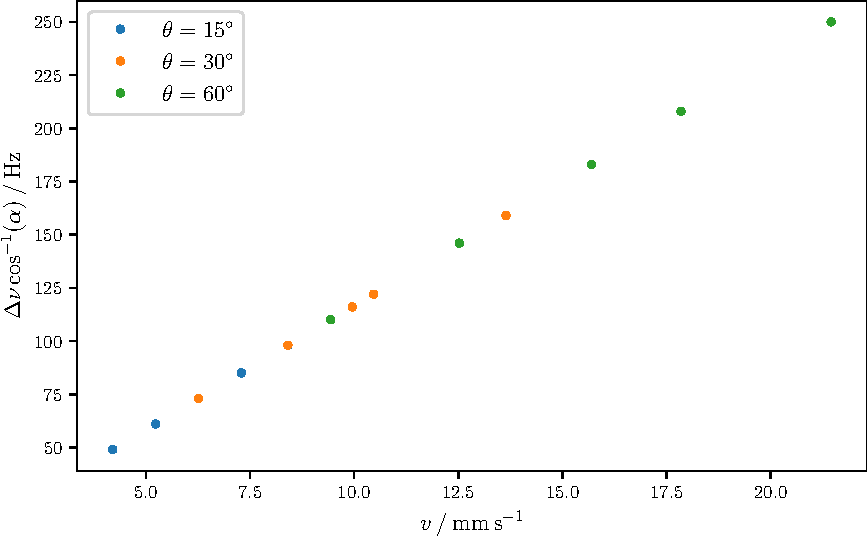
\includegraphics{build/big.pdf}
\end{figure}
\begin{figure}
    \centering
    \caption(Quotient gegen die Strömungsgeschwindigkeit des mittleren Rohrs)
    \label{fig:middle}
    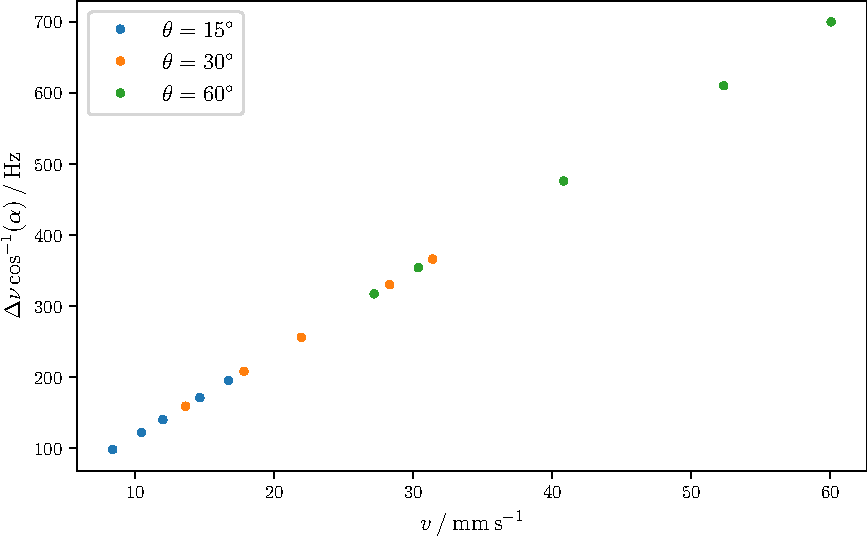
\includegraphics{build/middle.pdf}
\end{figure}
\begin{figure}
    \centering
    \caption(Quotient gegen die Strömungsgeschwindigkeit des dünnen Rohrs)
    \label{fig:tiny}
    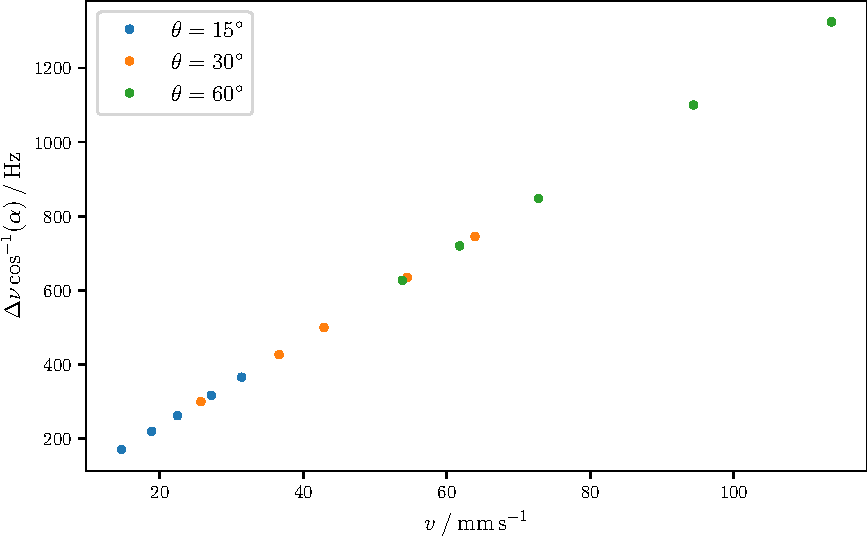
\includegraphics{build/tiny.pdf}
\end{figure}
\FloatBarrier
\subsection{Bestimmung des Strömungsprofils} \label{sec:profile}
Die Strömungsgeschwindigkeiten lassen sich erneut gemäß der Beziehung $REFERENZ$ ermitteln. 
In der Tabelle \ref{tab:profile} sind die gemessenen Frequenzverschiebungen und Streuintesitäten mit den errechneten Strömungsgeschwindigkeiten in Abhängigkeit
der Tiefe aufgezeichnet.
Die dazu erstellten Abbildungen \ref{fig:velocity} und \ref{fig:intensity} stellen einerseits das Geschwindigkeitsprofil und die Streuintesitäten in Abhängigkeit
der Messtiefe graphisch dar. Dabei sind die Messdaten bei den beiden Pump-Drehzahlen $6110 \, \text{rpm}$ und $5040 \, \text{rpm}$ aufgetragen. 
\begin{table}
    \centering
    \caption{Gemessene Frequenzverschiebungen und Streuintesität mit den errechneten Strömungsgeschwindigkeiten bei variierter Tiefe}
    \label{tab:profile}
    \begin{tabular}{S[table-format=2.1]
                    S[table-format=3.0] S[table-format=2.0] S[table-format = 2.3]
                    S[table-format=2.0] S[table-format=2.0] S[table-format = 2.3]}
        \toprule 
        &
        \multicolumn{3}{c}{$\num{6110} \, \text{rpm}$} &
        \multicolumn{3}{c}{$\num{5040} \, \text{rpm}$} \\
        \cmidrule(lr){2-4} \cmidrule(lr){5-7}
        {$d \mathbin{/} \si{\micro\second}$}&
        {$\symup{\Delta} \nu \mathbin{/} \si{\hertz}$} & {$I$} & {$v \mathbin{/} \si{\milli\metre\second\tothe{-1}}$} &
        {$\symup{\Delta} \nu \mathbin{/} \si{\hertz}$} & {$I$} & {$v \mathbin{/} \si{\milli\metre\second\tothe{-1}}$} \\
        \midrule
        13   & 0   & 5  & 0     & 0  & 10 & 0      \\
        13.5 & 0   & 12 & 0     & 0  & 10 & 0      \\
        14   & 0   & 22 & 0     & 0  & 10 & 0      \\
        14.5 & 0   & 27 & 0     & 0  & 20 & 0      \\
        15   & 0   & 45 & 0     & 0  & 26 & 0      \\
        15.5 & 146 & 70 & 72.6  & 0  & 25 & 0      \\
        16   & 153 & 68 & 76.081& 0  & 25 & 0      \\
        16.5 & 143 & 70 & 71.108& 0  & 20 & 0      \\
        17   & 143 & 56 & 71.108& 0  & 18 & 0      \\
        17.5 & 0   & 30 & 0     & 0  & 29 & 0      \\
        18   & 0   & 5  & 0     & 98 & 60 & 48.731 \\
        18.5 & 0   & 19 & 0     & 85 & 60 & 42.267 \\
        19   & 0   & 23 & 0     & 85 & 60 & 42.267 \\
    \end{tabular}
\end{table}
\begin{figure}
    \centering
    \caption(Geschwindigkeitsprofil bei 2 verschiedenen Drehzahlen)
    \label{fig:velocity}
    \includegraphics{build/velocity.pdf}
\end{figure}
\begin{figure}
    \centering
    \caption(Streuintesitäten bei 2 verschiedenen Drehzahlen)
    \label{fig:intensity}
    \includegraphics{build/intensity.pdf}
\end{figure}
Normalerweise würde man ein Strömungprofil erwarten, welches nah an der Rohrwand aufgrund der Viskosität der Flüssigkeit langsamer wäre und zu der Mitte des 
Rohrs hin höhere Geschwindigkeiten aufweist.
Jedoch lässt sich dort nicht solch eine Struktur aufweisen, da es trotz den mutmaßlich richtigen Tiefen zu keiner Frequenzverschiebungen kam.
Somit lässt sich bei diesen Tiefen eine Strömungsgeschwindigkeit von $\SI{0}{\metre\per\second}$ errechnen.
Die Ursaschen für diese Messwerte werden im weitern Verlauf in Abschnitt \ref{sec:Diskussion} disskutiert.